\documentclass[letterpaper]{article}
\usepackage{geometry}
\geometry{margin=1.1in}
\usepackage[protrusion=true,expansion=true]{microtype}	
\usepackage[boxruled,linesnumbered,vlined,inoutnumbered]{algorithm2e}
\usepackage{amsmath}
\usepackage{amsthm}
\usepackage{amssymb}
\usepackage{mathtools}
\usepackage{mathrsfs}
\usepackage{soul}
\usepackage{natbib}
\usepackage{rotating}
\usepackage{gensymb}
\usepackage{lscape}
\usepackage{array}
\usepackage{makecell}
\renewcommand\theadalign{bc}
\renewcommand\theadfont{\bfseries}
\renewcommand\theadgape{\Gape[4pt]}
\renewcommand\cellgape{\Gape[4pt]}
\usepackage{courier}
\usepackage{lipsum}
\usepackage{graphicx}
\usepackage{subcaption}
\usepackage[space]{grffile}
\usepackage{xcolor}
\definecolor{light-grey}{rgb}{0.9,0.9,0.9}
\definecolor{dark-red}{rgb}{0.4,0.15,0.15}
\definecolor{dark-blue}{rgb}{0,0,0.7}
\usepackage{environ}
\setcounter{tocdepth}{2}
\renewcommand{\contentsname}{Table of Contents}
\usepackage{hyperref}
\hypersetup{
    colorlinks, linkcolor={dark-blue},
    citecolor={dark-blue}, urlcolor={dark-blue}
}

\setlength{\parskip}{1em}
\newcommand{\HIGHLIGHT}[1]{\textcolor{blue}{\textbf{#1}}}
\newcommand{\TODO}[1]{\textcolor{red}{\textbf{#1}}}

\begin{document}
%-----------------
%	Homework 4
%-----------------
\newpage
\section*{Calvin Cuff}
\begin{center}
    \begin{Large}
    COMPSCI 589 Homework 4 - Spring 2025
    \end{Large}
    \\
    \HIGHLIGHT{Due May 01, 2025, 11:59pm Eastern Time}
\end{center}
\addcontentsline{toc}{subsection}{\textbf{Homework 4}}



% \vspace{0.15in}
\section*{Programming Section (100 Points Total)}

\textbf{Deliverables and Experiments}

The main objective of this homework is to study how the performance of a trained neural network is affected by \textit{(i)} the neural network architecture (i.e., by the number of layers and neurons); and \textit{(ii)} by the regularization parameter. 

When implementing your neural network, do not forget to add a \textit{bias} input to each neuron, and to ensure that updates to bias weights are performed correctly if regularization is used. For more information, please see the slides of the corresponding lecture. Also, do not forget to properly normalize the attributes of training and test instances whenever appropriate/necessary. 

You are free to choose between two simple stopping criteria. You may, for instance, \textit{(1)} stop if (after presenting all training instances to the network and updating its weights) the cost function $J$ improves by less than some small user-adjusted constant $\epsilon$; or  \textit{(2)} stop after a constant, pre-defined number $m$ of iterations---where each iteration consists of presenting all instances of the training set to the network, computing gradients, and updating the network's weights. You are free to choose which criterion you would like to use. \textit{In all questions below, do not forget to mention explicitly which criterion you used and what was its corresponding hyper-parameter (i.e., $\epsilon$ or $m$). We encourage you to try different possibilities to identify the setting that produces the best possible performance for your algorithm.}

\underline{After} verifying and ensuring the correctness of your solution (by comparing the outputs produced by your backpropagation implementation with the step-by-step examples we provided; please see Section \ref{correctness_verif}), you will be analyzing two datasets. \textbf{Both datasets can be found in this homework's ``Supporting Files'' zip file on Canvas.}

\textbf{(1) The Wisconsin Breast Cancer Diagnostic (WDBC) Dataset.}
The goal here is to train a classifier capable of predicting whether a breast mass is malignant or benign, based on features computed from a digitized image of a breast mass. The dataset is composed of 569 instances. Each instance is described by 30 \textit{numerical} attributes, and there are two classes.

\textbf{(2) The Loan Eligibility Prediction Dataset.}
Here, the goal is to automatically (and accurately) predict whether a given person should qualify for a loan. Each instance is described by 11 attributes, including the gender of the applicant, whether the applicant is married, their income, information about their credit history, etc. The binary target class to be predicted is whether a given applicant's request for a loan was approved or not. Notice that this dataset contains 7 \textit{categorical} attributes and 4 \textit{numerical} attributes. There is a total of 480 instances in the dataset. 

%\vspace{1cm}
\noindent\rule{\textwidth}{1pt}
\noindent $\star$ \textcolor{violet}{Notice that some of the datasets above include both categorical and numerical attributes. Algorithms such as neural networks (as well as others) require numerical inputs. The standard way of converting categorical inputs to numerical inputs is by using the \textit{one-hot encoding} technique. For a quick and high-level introduction to one-hot encoding, as well as examples on how to use Scikit's libraries to perform this type of conversion, please visit this \href{https://datagy.io/sklearn-one-hot-encode}{website}}.\\
\noindent\rule{\textwidth}{1pt}
%\vspace{1cm}



\section{Correctness Verification}
\label{correctness_verif}
\subsection{Backpropagation Example 1}

\begin{verbatim}
tom@W1188YW8Y3:~/umass/ml_cs589/neural_net$ python3 backprop_example1.py 
X [[0.13]
 [0.42]]
y [[0.9 ]
 [0.23]]
DEBUG:neural_network.neural_network:x: [0.13]
DEBUG:neural_network.neural_network:a1: [1.   0.13]
DEBUG:neural_network.neural_network:z2: [0.413 0.326]
DEBUG:neural_network.neural_network:a2: [1.        0.601807  0.5807858]
DEBUG:neural_network.neural_network:z3: [1.34937498]
DEBUG:neural_network.neural_network:a3: [0.79402743]
DEBUG:neural_network.neural_network:f(x): [0.79402743]
DEBUG:neural_network.neural_network:Cost: 0.36557475812121376

DEBUG:neural_network.neural_network:delta3: [-0.10597257]
DEBUG:neural_network.neural_network:grads2: [[-0.10597257 -0.06377504 -0.06154737]]
DEBUG:neural_network.neural_network:delta2: [-0.01269739 -0.01548092]
DEBUG:neural_network.neural_network:grads1: [[-0.01269739 -0.00165066]
 [-0.01548092 -0.00201252]]
DEBUG:neural_network.neural_network:x: [0.42]
DEBUG:neural_network.neural_network:a1: [1.   0.42]
DEBUG:neural_network.neural_network:z2: [0.442 0.384]
DEBUG:neural_network.neural_network:a2: [1.         0.60873549 0.59483749]
DEBUG:neural_network.neural_network:z3: [1.36127024]
DEBUG:neural_network.neural_network:a3: [0.79596607]
DEBUG:neural_network.neural_network:f(x): [0.79596607]
DEBUG:neural_network.neural_network:Cost: 1.2763767660603886

DEBUG:neural_network.neural_network:delta3: [0.56596607]
DEBUG:neural_network.neural_network:grads2: [[0.56596607 0.34452363 0.33665784]]
DEBUG:neural_network.neural_network:delta2: [0.06739994 0.08184068]
DEBUG:neural_network.neural_network:grads1: [[0.06739994 0.02830797]
 [0.08184068 0.03437309]]

Regularized Loss over all training samples 0.8209757620908011

Final grads of theta1
 [[0.02735127 0.01332866]
 [0.03317988 0.01618028]]

Final grads of theta2
 [[0.22999675 0.1403743  0.13755523]]
\end{verbatim}
\clearpage


\subsection{Backpropagation Example 2}
\begin{verbatim}
tom@W1188YW8Y3:~/umass/ml_cs589/neural_net$ python3 backprop_example2.py 
X [[0.32 0.68]
 [0.83 0.02]]
y [[0.75 0.98]
 [0.75 0.28]]
DEBUG:neural_network.neural_network:x: [0.32 0.68]
DEBUG:neural_network.neural_network:a1: [1.   0.32 0.68]
DEBUG:neural_network.neural_network:z2: [0.74   1.1192 0.3564 0.8744]
DEBUG:neural_network.neural_network:a2: [1.         0.67699586 0.75384029 0.5881687  0.70566042]
DEBUG:neural_network.neural_network:z3: [1.94769138 2.12135808 1.48153575]
DEBUG:neural_network.neural_network:a3: [1.         0.87519469 0.89296181 0.81480444]
DEBUG:neural_network.neural_network:z4: [1.60830969 1.66804824]
DEBUG:neural_network.neural_network:a4: [0.83317658 0.84131543]
DEBUG:neural_network.neural_network:f(x): [0.83317658 0.84131543]
DEBUG:neural_network.neural_network:Cost: 0.7907366592171865

DEBUG:neural_network.neural_network:delta4: [ 0.08317658 -0.13868457]
DEBUG:neural_network.neural_network:grads3: [[ 0.08317658  0.0727957   0.07427351  0.06777264]
 [-0.13868457 -0.121376   -0.12384003 -0.1130008 ]]
DEBUG:neural_network.neural_network:delta3: [ 0.00638937 -0.00925379 -0.00778767]
DEBUG:neural_network.neural_network:grads2: [[ 0.00638937  0.00432557  0.00481656  0.00375802  0.00450872]
 [-0.00925379 -0.00626478 -0.00697588 -0.00544279 -0.00653003]
 [-0.00778767 -0.00527222 -0.00587066 -0.00458046 -0.00549545]]
DEBUG:neural_network.neural_network:delta2: [-0.00086743 -0.00133354 -0.00053312 -0.00070163]
DEBUG:neural_network.neural_network:grads1: [[-0.00086743 -0.00027758 -0.00058985]
 [-0.00133354 -0.00042673 -0.00090681]
 [-0.00053312 -0.0001706  -0.00036252]
 [-0.00070163 -0.00022452 -0.00047711]]
DEBUG:neural_network.neural_network:x: [0.83 0.02]
DEBUG:neural_network.neural_network:a1: [1.   0.83 0.02]
DEBUG:neural_network.neural_network:z2: [0.5525 0.8138 0.1761 0.6041]
DEBUG:neural_network.neural_network:a2: [1.         0.63471542 0.69291867 0.54391158 0.64659376]
DEBUG:neural_network.neural_network:z3: [1.81695963 2.02468436 1.373268  ]
DEBUG:neural_network.neural_network:a3: [1.         0.86020091 0.88336451 0.79790763]
DEBUG:neural_network.neural_network:z4: [1.58227893 1.64577265]
DEBUG:neural_network.neural_network:a4: [0.82952703 0.83831889]
DEBUG:neural_network.neural_network:f(x): [0.82952703 0.83831889]
DEBUG:neural_network.neural_network:Cost: 1.943782263716031

DEBUG:neural_network.neural_network:delta4: [0.07952703 0.55831889]
DEBUG:neural_network.neural_network:grads3: [[0.07952703 0.06840922 0.07025135 0.06345522]
 [0.55831889 0.48026642 0.4931991  0.44548691]]
DEBUG:neural_network.neural_network:delta3: [0.01503437 0.05808969 0.06891698]
DEBUG:neural_network.neural_network:grads2: [[0.01503437 0.00954254 0.01041759 0.00817737 0.00972113]
 [0.05808969 0.03687042 0.04025143 0.03159565 0.03756043]
 [0.06891698 0.04374267 0.04775386 0.03748474 0.04456129]]
DEBUG:neural_network.neural_network:delta2: [0.01694006 0.01465141 0.01998824 0.01622017]
DEBUG:neural_network.neural_network:grads1: [[0.01694006 0.01406025 0.0003388 ]
 [0.01465141 0.01216067 0.00029303]
 [0.01998824 0.01659024 0.00039976]
 [0.01622017 0.01346274 0.0003244 ]]

Regulaized Loss over all training samples 1.9035094614666088

Final grads of theta1
 [[0.00803632 0.02564134 0.04987447]
 [0.00665894 0.01836697 0.06719311]
 [0.00972756 0.03195982 0.05251862]
 [0.00775927 0.05036911 0.08492365]]

Final grads of theta2
 [[0.01071187 0.09068406 0.02511708 0.1259677  0.11586492]
 [0.02441795 0.06780282 0.04163777 0.05307643 0.1267652 ]
 [0.03056466 0.08923522 0.1209416  0.10270214 0.03078292]]

Final grads of theta3
 [[0.0813518  0.17935246 0.12476243 0.13186393]
 [0.20981716 0.19194521 0.30342954 0.25249305]]
\end{verbatim}
\clearpage

\section{Experiments and Analyses}
\subsection{WDBC}

For experiments with the WDBC dataset, I performed a grid search over various network architectures and regularization strengths. Through preliminary testing, I identified a learning rate of 1e-1 as the most effective, and this value was used for all subsequent experiments. A fixed number of training iterations was used as the stopping criterion: the training process was terminated after presenting the full training set 500 times.

\begin{enumerate}
    \item \textbf{Hyper Parameter Search Results}

    Using stratified cross validation, I tested neural network architectures with hidden layers consisting of [10], [20], [40], [20,10], [30,15], and [40,20,10] neurons. For each network architecture I also tweaked the regularization strength, experimenting with values of 0, 1e-3, 1e-2, and 1e-1.

    % Requires: \usepackage{array}
\begin{table}[h]
    \centering
    \begin{tabular}{|>{\raggedright\arraybackslash}p{3cm}|>{\raggedright\arraybackslash}p{3cm}|>{\raggedright\arraybackslash}p{3cm}|>{\raggedright\arraybackslash}p{3cm}|}
    \hline
    Regularization Strength & Hidden Dimensions & Accuracy & F1 Score \\ \hline
    0.0 & [10] & 0.8681 & 0.908 \\ \hline
    0.0 & [20] & 0.9275 & 0.946 \\ \hline
    0.0 & [40] & 0.9341 & 0.9507 \\ \hline
    0.0 & [20, 10] & 0.6352 & 0.7769 \\ \hline
    0.0 & [30, 15] & 0.6374 & 0.7779 \\ \hline
    0.0 & [40, 20, 10] & 0.6352 & 0.7769 \\ \hline
    0.001 & [10] & 0.9077 & 0.9327 \\ \hline
    0.001 & [20] & 0.9187 & 0.9398 \\ \hline
    0.001 & [40] & 0.9297 & 0.9475 \\ \hline
    0.001 & [20, 10] & 0.6352 & 0.7769 \\ \hline
    0.001 & [30, 15] & 0.6396 & 0.779 \\ \hline
    0.001 & [40, 20, 10] & 0.6352 & 0.7769 \\ \hline
    0.01 & [10] & 0.8769 & 0.9122 \\ \hline
    0.01 & [20] & 0.9099 & 0.9338 \\ \hline
    \textbf{0.01} & \textbf{[40]} & \textbf{0.9407} & \textbf{0.9554} \\ \hline
    0.01 & [20, 10] & 0.6374 & 0.7779 \\ \hline
    0.01 & [30, 15] & 0.6352 & 0.7769 \\ \hline
    0.01 & [40, 20, 10] & 0.6352 & 0.7769 \\ \hline
    0.1 & [10] & 0.8813 & 0.9159 \\ \hline
    0.1 & [20] & 0.9187 & 0.9397 \\ \hline
    0.1 & [40] & 0.9319 & 0.9491 \\ \hline
    0.1 & [20, 10] & 0.6396 & 0.779 \\ \hline
    0.1 & [30, 15] & 0.6352 & 0.7769 \\ \hline
    0.1 & [40, 20, 10] & 0.6352 & 0.7769 \\ \hline
    \end{tabular}
    \caption{Validation Accuracy and F1 Score across different Regularization Strengths and Hidden Layer Configurations (WDBC)}
\end{table}
\clearpage



    \item \textbf{Discuss (on a high level) what contributed the most to improving performance.}
    
    For the WDBC dataset, model performance was most sensitive to the number of neurons used in the hidden layer. Using a single hidden layer yielded the best results with my training strategy, and performance consistently improved as the number of neurons in that layer increased. The model performed reasonably well with 10 neurons, better with 20 neurons, and achieved the best results with 40 neurons in the hidden layer. However, when additional hidden layers were introduced, performance dropped off sharply, suggesting that increasing network complexity actually hindered the learning process. This degradation could potentially be mitigated by extending the training duration or adjusting other hyperparameters.

    
 \item \textbf{Discuss which neural network architecture you would deploy in real life.} 

    Based on the results of the previous experiments I would deploy a neural network architecture consisting of a single hidden layer with 40 neurons, using a regularization strength of 1e-2, and a learning rate of 1e-1. This network and associated hyperparameters achieved the highest validation accuracy (94.07\%) and F1 Score (0.9554) across all tested models with a standardizes training setup. The results indicate that this architecture captures the best balance between model complexity and generalization performance. Increasing the number of neurons in a single hidden layer allowed the network to better capture the underlying structure of the data without overfitting. Adding additional hidden layers introduced unnecessary complexity, which degraded performance significantly.
 
\item \textbf{Test Loss Learning Curve}

    The following graph shows the results of training the best model identified from previous experiments on varying amounts of the training data, reporting the test loss at each stage of the training. The model configuration for this experiment was a neural network consisting of a single hidden layer with 40 neurons, a regularization rate of 1e-2 and a learning rate of 1e-1.

     \vspace{0.2in}
        \begin{minipage}{\linewidth}
            \centering
            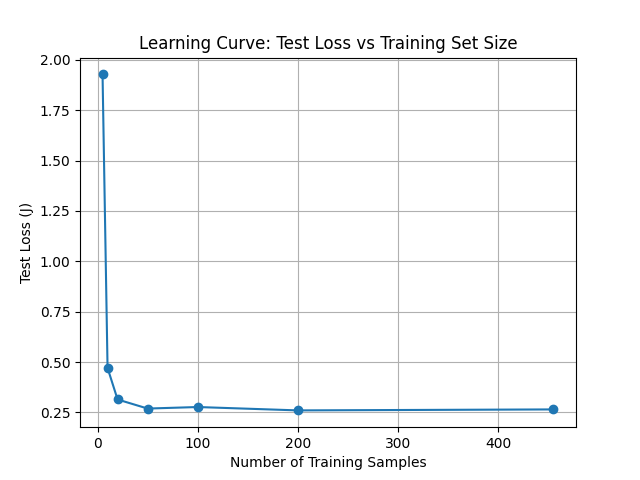
\includegraphics[width=10cm]{figures/wdbc_test_loss.png}
            \captionof{figure}{Test loss vs training size on wdbc.csv dataset}
        \end{minipage}
        \vspace{0.1in}

        
\end{enumerate}

\newpage
\subsection{Loan}

For experiments with the Loan dataset, I performed a grid search over various network architectures and regularization strengths. Through preliminary testing, I identified a learning rate of 1e-1 as the most effective, and this value was used for all subsequent experiments. A fixed number of training iterations was used as the stopping criterion: the training process was terminated after presenting the full training set 3000 times.

\begin{enumerate}
    \item \textbf{Hyper Parameter Search Results}

     Using stratified cross validation, I tested neural network architectures with hidden layers consisting of [2], [4], [10], [20], [40], [20,10], [30,15], and [40,20,10] neurons. For each network architecture I also tweaked the regularization strength, experimenting with values of 0, 1e-3, 1e-2, and 1e-1.
     
    \begin{table}[h]
    \centering
    \begin{tabular}{|>{\raggedright\arraybackslash}p{3cm}|>{\raggedright\arraybackslash}p{3cm}|>{\raggedright\arraybackslash}p{3cm}|>{\raggedright\arraybackslash}p{3cm}|}
    \hline
    Regularization Strength & Hidden Dimensions & Accuracy & F1 Score \\ \hline
    0.0 & [2] & 0.8046 & 0.873 \\ \hline
    0.0 & [4] & 0.8046 & 0.8727 \\ \hline
    0.0 & [10] & 0.8021 & 0.8714 \\ \hline
    0.0 & [20] & 0.8098 & 0.8765 \\ \hline
    0.0 & [40] & 0.8124 & 0.8784 \\ \hline
    0.0 & [20, 10] & 0.8124 & 0.8784 \\ \hline
    0.0 & [30, 15] & 0.8099 & 0.877 \\ \hline
    0.0 & [40, 20, 10] & 0.8072 & 0.8751 \\ \hline
    0.001 & [2] & 0.8098 & 0.8769 \\ \hline
    0.001 & [4] & 0.8072 & 0.875 \\ \hline
    0.001 & [10] & 0.8124 & 0.878 \\ \hline
    0.001 & [20] & 0.8072 & 0.8745 \\ \hline
    0.001 & [40] & 0.802 & 0.8708 \\ \hline
    0.001 & [20, 10] & 0.8098 & 0.8765 \\ \hline
    0.001 & [30, 15] & 0.8046 & 0.8728 \\ \hline
    0.001 & [40, 20, 10] & 0.8072 & 0.8747 \\ \hline
    0.01 & [2] & 0.8177 & 0.8823 \\ \hline
    0.01 & [4] & 0.8124 & 0.8785 \\ \hline
    0.01 & [10] & 0.8098 & 0.8769 \\ \hline
    0.01 & [20] & 0.8124 & 0.8789 \\ \hline
    0.01 & [40] & 0.815 & 0.8803 \\ \hline
    0.01 & [20, 10] & 0.8098 & 0.8766 \\ \hline
    0.01 & [30, 15] & 0.8177 & 0.8822 \\ \hline
    \textbf{0.01} & \textbf{[40, 20, 10]} & \textbf{0.8203} & \textbf{0.8841} \\ \hline
    0.1 & [2] & 0.7943 & 0.8639 \\ \hline
    0.1 & [4] & 0.7969 & 0.8659 \\ \hline
    0.1 & [10] & 0.7891 & 0.8603 \\ \hline
    0.1 & [20] & 0.7917 & 0.8619 \\ \hline
    0.1 & [40] & 0.7969 & 0.8654 \\ \hline
    0.1 & [20, 10] & 0.7917 & 0.8615 \\ \hline
    0.1 & [30, 15] & 0.7943 & 0.8634 \\ \hline
    0.1 & [40, 20, 10] & 0.7917 & 0.8615 \\ \hline
    \end{tabular}
    \caption{Validation Accuracy and F1 Score across different Regularization Strengths and Hidden Layer Configurations (Loan)}
\end{table}
\clearpage


    \item \textbf{Discuss (on a high level) what contributed the most to improving performance.}

    Tuning the hyperparameters for this dataset proved to be much more challenging, as the performance remained fairly consistent across the different architectures and regularization strengths. There were minimal differences in validation accuracy and F1 score, regardless of the number of network layers or number of neurons.
    
     Adding more neurons to a single layer did not lead to significant improvements or decrease the performance. Adding deeper layers to the network, 2 or 3 for example, did not show a strong correlation to increased model performance or learning capability. 

    The model also showed a strong insensitivity to regularization strength. 
    With no regularization or weak regularization values (1e-2, 1e-3) the model performance was stable. When the regularization strength was increased to 1e-1, the model performed its worse across all architectures - although it was a minimal decrease.

 \item \textbf{Discuss which neural network architecture you would deploy in real life.} 

     Based on the results of the previous experiments I would deploy a neural network architecture consisting of 3 hidden layers with 40, 20, and 10 neurons, respectively. I would also use a regularization strength of 1e-2 and a learning rate of 1e-1. This network and associated hyperparameters achieved its highest validation accuracy (82.03\%) and F1 Score (0.8841) across all tested models with a standardized training setup. The results indicate that this architecture captures the best balance between model complexity and generalization performance. This data set proved to be the most difficult to see performance improvements so it makes sense to deploy the more sophisticated model with deeper layers and more neurons, capable of capturing more complex relationships from the data.
     

\item \textbf{Test Loss Learning Curve}

    The following graph shows the results of training the best model identified from previous experiments on varying amounts of the training data, reporting the test loss at each stage of the training. The model configuration for this experiment was a neural network consisting of 3 hidden layers with 40, 20, and 10 neurons, respectively, a regularization rate of 1e-2 and a learning rate of 1e-1.

     \vspace{0.2in}
        \begin{minipage}{\linewidth}
            \centering
            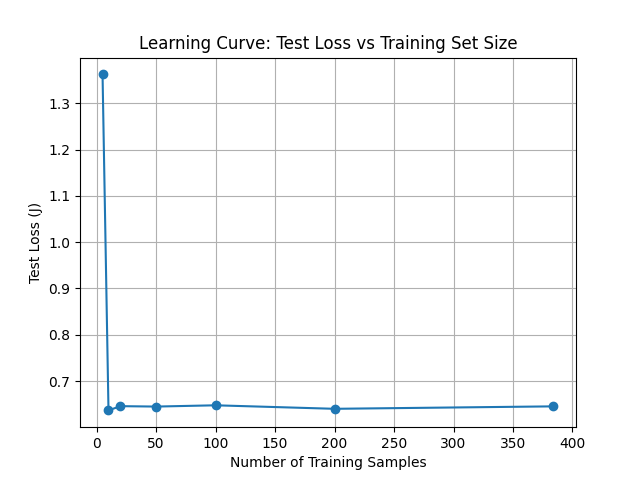
\includegraphics[width=10cm]{figures/loan_test_loss.png}
            \captionof{figure}{Test loss vs training size on loan.csv dataset}
        \end{minipage}
        \vspace{0.1in}

\end{enumerate}

\newpage

\newpage
\subsection{Raisin}

For experiments with the Raisin dataset, I performed a grid search over various network architectures and regularization strengths. Through preliminary testing, I identified a learning rate of 1e-1 as the most effective, and this value was used for all subsequent experiments. A fixed number of training iterations was used as the stopping criterion: the training process was terminated after presenting the full training set 1000 times.

\begin{enumerate}
    \item \textbf{Hyper Parameter Search Results}

     Using stratified cross validation, I tested neural network architectures with hidden layers consisting of [2], [4], [10], [20], [40], [2,2], [20,10], [30,15], and [40,20,10] neurons. For each network architecture I also tweaked the regularization strength, experimenting with values of 0, 1e-3, 1e-2, and 1e-1.

    \begin{table}[h]
    \centering
    \begin{tabular}{|>{\raggedright\arraybackslash}p{3cm}|>{\raggedright\arraybackslash}p{3cm}|>{\raggedright\arraybackslash}p{3cm}|>{\raggedright\arraybackslash}p{3cm}|}
    \hline
    Regularization Strength & Hidden Dimensions & Accuracy & F1 Score \\ \hline
    0.0 & [2] & 0.7861 & 0.8119 \\ \hline
    0.0 & [10] & 0.8569 & 0.8514 \\ \hline
    0.0 & [20] & 0.8611 & 0.8568 \\ \hline
    0.0 & [40] & 0.8653 & 0.8614 \\ \hline
    0.0 & [2, 2] & 0.6833 & 0.6759 \\ \hline
    0.0 & [20, 10] & 0.8653 & 0.8580 \\ \hline
    0.0 & [30, 15] & 0.8472 & 0.8404 \\ \hline
    0.0 & [40, 20, 10] & 0.7542 & 0.6420 \\ \hline
    0.001 & [2] & 0.8431 & 0.8335 \\ \hline
    0.001 & [10] & 0.8597 & 0.8548 \\ \hline
    0.001 & [20] & 0.8597 & 0.8545 \\ \hline
    0.001 & [40] & 0.8653 & 0.8623 \\ \hline
    0.001 & [2, 2] & 0.7056 & 0.7059 \\ \hline
    0.001 & [20, 10] & 0.8403 & 0.8250 \\ \hline
    0.001 & [30, 15] & 0.8528 & 0.8431 \\ \hline
    0.001 & [40, 20, 10] & 0.8250 & 0.8093 \\ \hline
    0.01 & [2] & 0.8611 & 0.8510 \\ \hline
    0.01 & [10] & 0.8556 & 0.8504 \\ \hline
    0.01 & [20] & 0.8653 & 0.8619 \\ \hline
    0.01 & [40] & 0.8611 & 0.8587 \\ \hline
    0.01 & [2, 2] & 0.6778 & 0.7310 \\ \hline
    0.01 & [20, 10] & 0.8528 & 0.8471 \\ \hline
    0.01 & [30, 15] & 0.8403 & 0.8305 \\ \hline
    0.01 & [40, 20, 10] & 0.7778 & 0.7889 \\ \hline
    0.1 & [2] & 0.7972 & 0.8138 \\ \hline
    0.1 & [10] & 0.8653 & 0.8601 \\ \hline
    0.1 & [20] & 0.8625 & 0.8579 \\ \hline
    \textbf{0.1} & \textbf{[40]} & \textbf{0.8681} & \textbf{0.8652} \\ \hline
    0.1 & [2, 2] & 0.6681 & 0.6663 \\ \hline
    0.1 & [20, 10] & 0.8611 & 0.8609 \\ \hline
    0.1 & [30, 15] & 0.8417 & 0.8258 \\ \hline
    0.1 & [40, 20, 10] & 0.8306 & 0.8345 \\ \hline
    \end{tabular}
    \caption{Validation Accuracy and F1-Score for Different Network Architectures and Regularization Strengths}
\end{table}

     
    \item \textbf{Discuss (on a high level) what contributed the most to improving performance.}

    For the raisin dataset, adding more neurons to a single hidden layer contributed the most to improving model performance. Networks with a single layer and an increasing number of neurons demonstrated improvements in both validation accuracy and F1 score. For example, expanding from just 2 neurons to 20 or 40 neurons consistently boosted performance. 

    Introducing additional layers with very few neurons per layers, such as [2,2], led to a decrease in performance. However introducing a second hidden layer with a moderate number of neurons produced comparable results to the single hidden layer with similar amount of neurons. Adding a third hidden layer, [40,20,10], resulted in a sharp decrease in validation performance, indicating this more sophisticated model was overly complex and did not learn the data patterns as well.

    This dataset was fairly resistant to changes in regularization strength. Wether using no regularization at all, small values such as 1e-3 and 1e-2, or stronger regularization, the model performance remained relatively stable.
    
     \item \textbf{Discuss which neural network architecture you would deploy in real life.} 
     
     Based on the results of the previous experiments I would deploy a neural network architecture consisting of a single hidden layer with 40 neurons, using a regularization strength of 1e-1, and a learning rate of 1e-1. 
     
     This network and associated hyperparameters achieved the highest validation accuracy (86.81\%) and F1 Score (0.8652) across all tested models with a standardizes training setup. The results indicate that this architecture captures the best balance between model complexity and generalization performance. Increasing the number of neurons in a single hidden layer allowed the network to better capture the underlying structure of the data without overfitting. Adding additional hidden layers with similar amounts of neurons introduced unnecessary complexity, that did not lead to enhanced model performance.

     

\item \textbf{Test Loss Learning Curve}

    The following graph shows the results of training the best model identified from previous experiments on varying amounts of the training data, reporting the test loss at each stage of the training. The model configuration for this experiment was a neural network consisting of a single hidden layer with 40 neurons, a regularization rate of 1e-1 and a learning rate of 1e-1.

     \vspace{0.2in}
        \begin{minipage}{\linewidth}
            \centering
            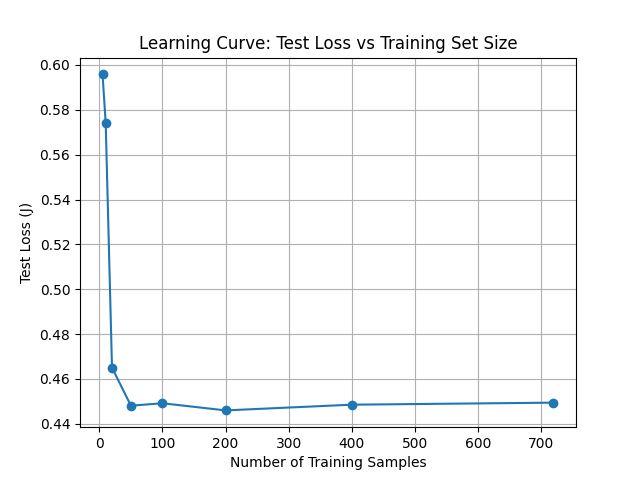
\includegraphics[width=10cm]{figures/raisin_test_loss.png}
            \captionof{figure}{Test loss vs training size on raisin.csv dataset}
        \end{minipage}
        \vspace{0.1in}

        
\end{enumerate}


\end{document}